\documentclass[9pt]{IEEEtran}

\usepackage[english]{babel}
\usepackage{graphicx}
\usepackage{epstopdf}
\usepackage{fancyhdr}
\usepackage{amsmath}
\usepackage{amsthm}
\usepackage{amssymb}
\usepackage{url}
\usepackage{array}
\usepackage{textcomp}
\usepackage{listings}
\usepackage{hyperref}
\usepackage{xcolor}
\usepackage{colortbl}
\usepackage{float}
\usepackage{gensymb}
\usepackage{longtable}
\usepackage{supertabular}
\usepackage{multicol}

\usepackage[utf8x]{inputenc}

\usepackage[T1]{fontenc}
\usepackage{lmodern}{}
\input{glyphtounicode}
\pdfgentounicode=1

\graphicspath{{./figures/}}
\DeclareGraphicsExtensions{.pdf,.png,.jpg,.eps}

% correct bad hyphenation here
\hyphenation{op-tical net-works semi-conduc-tor trig-gs}

% ============================================================================================

\title{\vspace{0ex}
Bayesian Inference}

\author{Marko Medved\vspace{-4.0ex}}

% ============================================================================================

\begin{document}

\maketitle

\section{Implementation of the Poisson GLM with Bayesian inference using MCMC}

\subsection{Implementation details}

For this part of the assignment we implemented the Poisson GLM with Bayesian 
inference. Firstly we standardized the data. Next, for 
our prior distribution of the regression coefficients ($\beta$ - as) we used 
the Normal distribution with large variance $\alpha = 10$. We chose this prior 
because then we don't have a real constraint on the bounds of the coefficients and 
the large variance makes the prior slightly more "uniform" so we don't really assume
that the coeficients are in a very specific area. To sample from our posterior 
we used the Markov Chain Monte Carlo (MCMC) method. To ensure robust computation 
of convergence diagnostics we used 4 independent chains. We sampled 3000 
samples from each chain with a burn-in period of 1000 samples. 

\subsection{Relationship between the explanatory and GoalsScored variables}
To describe the relationship between the features and the target variable we 
plot the densities of the posteriors of the regression coefficients on Figure~\ref{fig:densities}.
We can see that with high probability the Score Rate of the home team is the most 
important feature, contributing obviously positively to the amout of goals scored. 
On the other hand the 


\begin{figure}[h]
\centering
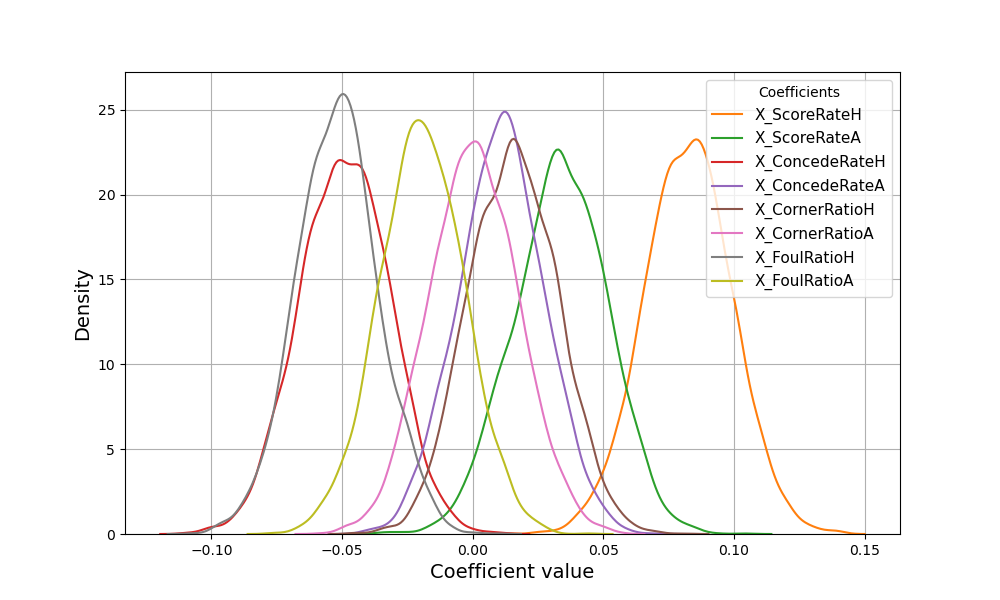
\includegraphics[width=1\columnwidth]{figures/densities.png}
\caption{Densities of coefficients for the features with the exclusion of the 
intercept density}
\label{fig:densities}
\end{figure}



\subsection{MCMC diagnostics}

\begin{figure}[h]
\centering
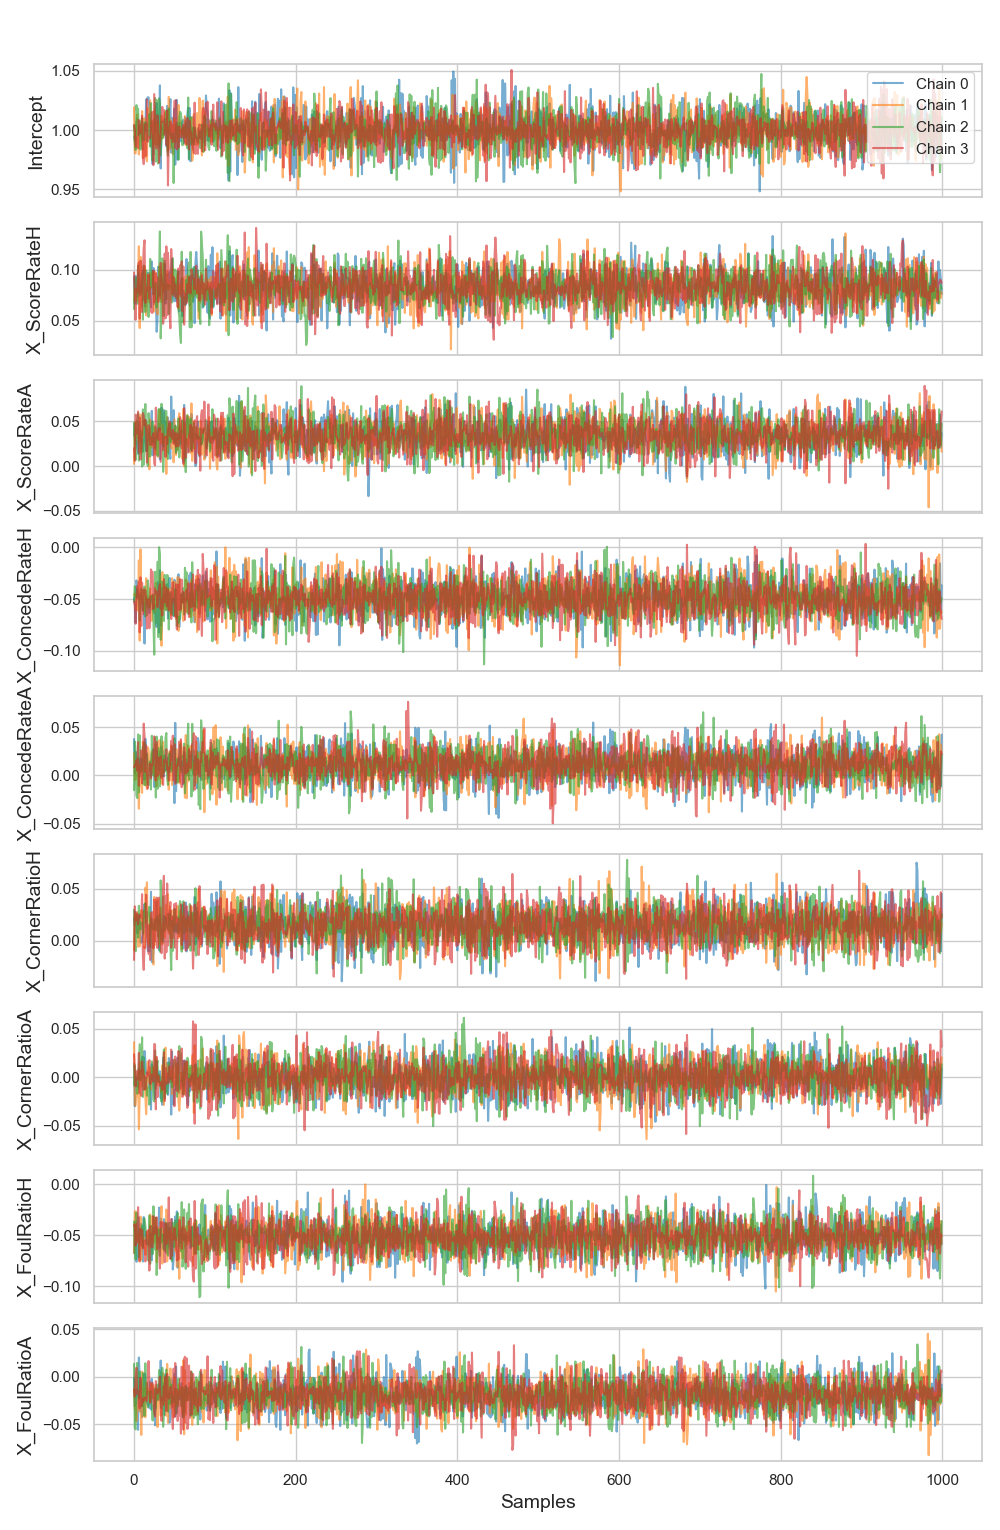
\includegraphics[width=1\columnwidth]{figures/trace.png}
\caption{}
\label{fig:trace}
\end{figure}


\begin{figure}[h]
\centering
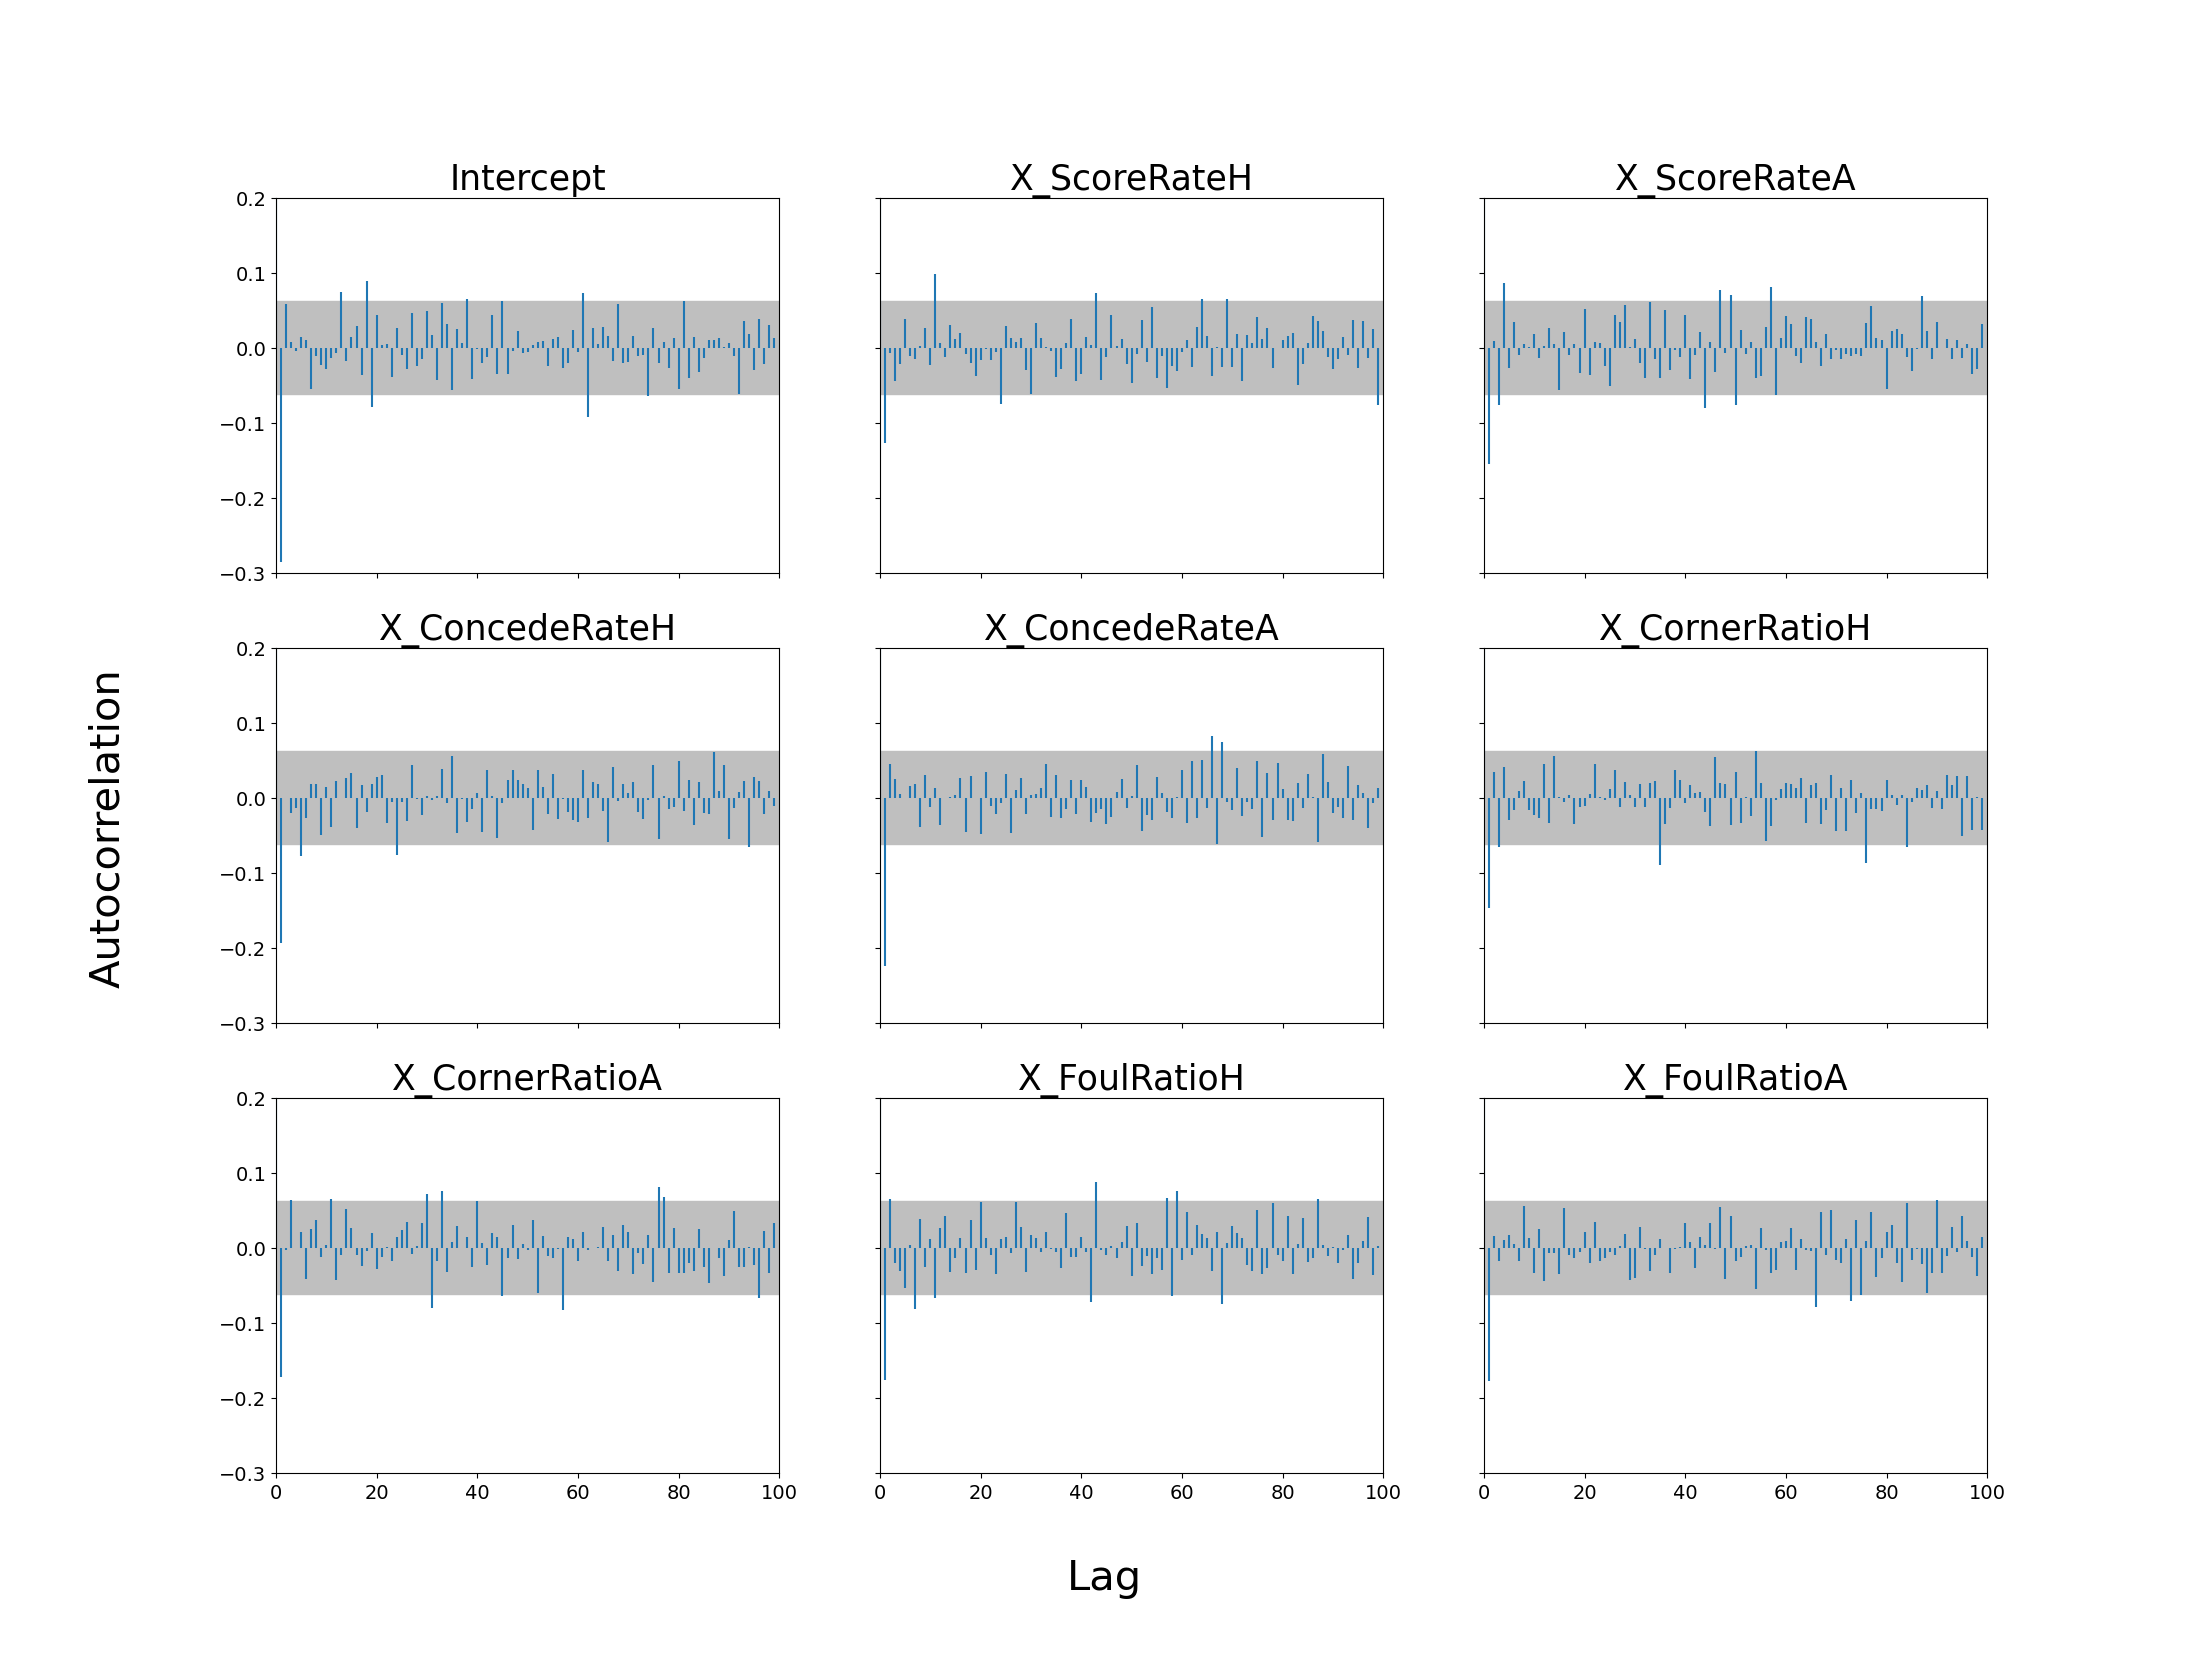
\includegraphics[width=1\columnwidth]{figures/autocorr.png}
\caption{}
\label{fig:autocorr}
\end{figure}






\bibliographystyle{IEEEtran}
\bibliography{bibliography}

\end{document}
